\chapter{Przegląd wybranych rozwiązań}
\section{Ruby on Rails}
Ruby on Rails jest open source'owym frameworkiem webowym. Został stworzony w~głównej mierze przez duńskiego programistę Davida Heinemeiera Hanssona. Pierwsza wersja RoR ukazała się w~lipcu 2004 roku. Fakt ten pokazuje, że jest to już dojrzały framework, z~ugruntowaną pozycją na rynku. Potwierdzeniem tej pozycji jest liczne wsparcie społeczności. Rails'y zostały stworzone przez ponad 4,5 tysiąca osób, istnieje ok. 132 tysiące ogólnodostępnych paczek, które rozszerzają funkcjonalność tego frameworku. Ruby on Rails domyślnie korzysta z~architektury MVC, czyli \emph{Model - View - Controller}.

\subsection{Doktryna Ruby on Rails}
Tworzeniu i~rozwojowi Ruby on Rails towarzyszy kilka podstawowych zasad. Jedne istnieją od początku, inne ewoluowały na przestrzeni lat. Spisane są one w~\emph{The Rails Doctrine} \cite{rails_doctrine}. Na potrzeby pracy zostaną omówione najważniejsze z nich.

\subsubsection{Optimize for programmer happiness}
Pierwsza reguła odnosi się mocno do języka, z~którego wywodzą się Rails'y. Sam fakt umieszczenia nazwy języka Ruby w~nazwie frameworku pokazuje jak ważny jest on dla całego projektu. Motywacją stworzenia języka Ruby była chęć dostarczenia programistom radości z~pisania kodu. w~momencie powstawania Ruby'ego, większość popularnych wtedy języków programowania narzucało sposób pisania bądź stosowało liczne ograniczenia w~sposobie pisania kodu. Ruby stał w~opozycji do tych zasad, dając programistom pełną dowolność w~sposobie tworzenia kodu.

Jako przykład owego ,,uwolnienia'' programisty podawana jest \emph{Zasada Najmniejszego Zaskoczenia} (ang. The Principle of Least Surprise).
\begin{lstlisting}[caption={Wyjście z~interpretera Ruby'ego.},language=Ruby]
$ irb
irb(main):001:0> exit
$ irb
irb(main):001:0> quit
\end{lstlisting}

\begin{lstlisting}[caption={Wyjście z~interpretera Python'a.},language=Python]
$ python
>>> exit
Use exit() or Ctrl-D (i.e. EOF) to exit
\end{lstlisting}
Ruby zaakceptuje oba polecenia opuszczenia interpretera. Python natomiast, pomimo odczytania intencji programisty (wyświetlenie instrukcji), opuści interpreter jedynie po wpisaniu komendy \emph{exit()} lub po użyciu kombinacji klawiszy \emph{Ctrl-D}, co oczywiście nie jest zgodne z~oczekiwaniami programisty.

Wzorując się na zasadach, na których powstawał Ruby, Rails'y również miały umilać życie programistom. Jako przykład jest podawana klasa \emph{Inflector}. Zapisane są w~niej reguły oraz wyjątki od reguł w~języku angielskim, które umożliwiają mapowanie klasy \emph{Comment} na tabelę \emph{Comments}, \emph{Person} na \emph{People} itp. Kolejnym przykładem może być dodatek do Ruby'owej klasy \emph{Array}, który poza dostępnym w~Rubym pierwszym elementem tablicy, umożliwia dostęp do kolejnych czterech elementów tablicy, poprzez wyrażenia \emph{Array\#second,~Array\#third} itd.

Oczywiście nie są to kluczowe cechy frameworku, ale stanowczo zaznaczają ważkość celu, którym jest przede wszystkim sprawianie radości z~tworzenia oprogramowania.

\subsubsection{Convention over Configuration}
Twórcy Ruby on Rails starają się kłaść mocny nacisk na prostotę używania ich narzędzia. Zamiast zrzucać na programistów ciągłe podejmowanie decyzji w~kwestiach mało istotnych, jak na przykład format klucza obcego w~bazie danych, Rails'y narzucają konwencję nazewnictwa. Oczywiście jest możliwość konfiguracji narzuconych przez framework konwencji, lecz jest to raczej rzadko spotykane, a~wręcz niewskazane. Zasada ta, poza zdjęciem odpowiedzialności za część decyzji z~barków programisty, przynosi również inne korzyści.

Dzięki ,,domyślnej'' konwencji, możliwe jest stworzenie głębszej abstrakcji, na której operuje framework. Przykładem może być zastosowanie wcześniej wymienionej klasy \emph{Inflector}. Jeśli możliwe jest zmapowanie klasy \emph{Person} na tabelę \emph{People}, to możliwe jest również zmapowanie relacji \emph{has\_many: people} w~taki sposób, aby wykorzystywana była klasa \textit{Person}. Jest to o~tyle wygodne rozwiązanie, że nawet pomimo posiadania wiedzy na temat tworzenia relacji w~bazie danych oraz sposobu odzwierciedlania ich w~kodzie aplikacji, programista nie musi przejmować się tworzeniem lub konfiguracją tej części aplikacji.

Kolejną zaletą jest znaczące obniżenie progu wejścia dla początkujących programistów. Takim osobom dużo łatwiej jest poznawać framework stopniowo. Począwszy od poziomu, gdzie wszystko automatycznie działa, lecz nie wiadomo dlaczego, aż do momentu gdzie nadal wszystko automatycznie działa, ale bardzo dobrze wiadomo dlaczego. Znaczna część mechanizmów stosowanych we frameworkach webowych \emph{de facto} nie wymaga niestandardowej konfiguracji, nawet jeśli programista posiada szeroką wiedzę w~danej dziedzinie. Przekładanie konfiguracji ponad konwencję wymaga od programisty sporego wysiłku, aby rozpocząć pracę z~frameworkiem, co w przypadku poznawania nowych technologii stanowczo nie jest zachęcające.

Zasada ta bywa jednak zgubna. Jest tak z~powodu błędnego przekonania, że skoro od samego początku wszystkie elementy aplikacji można wygenerować, i~od samego początku wszystko działa, to programista nie musi mieć wiedzy na temat tego, co robi. W~przypadku bardzo podstawowych zastosowań wiedza programisty rzeczywiście nie musi być szeroka, natomiast bardzo problematyczne jest w~takim przypadku wykonanie części aplikacji, która jest niestandardowa bądź niemożliwa do wygenerowania.

\subsubsection{The menu is omakase}
Rzadko kiedy framework jest monolitem, który nie składa się z~modułów. Częściej framework jest zbiorem mniejszych frameworków lub bibliotek, które współpracują ze sobą. Bardzo często wybór owych narzędzi leży w~pełni po stronie programisty. Jako analogię takiego wyboru, w \emph{The Ruby on Rails Doctrine} podawany jest problem wyboru dania z~menu w~restauracji, którą odwiedzamy po raz pierwszy. Jeśli zdamy się na wybór szefa kuchni, możemy założyć że jedzenie będzie dobre, nie wiedząc jeszcze co ,,dobre'' będzie oznaczać \cite{rails_doctrine}.

Ruby on Rails rozwiązuje ten problem poprzez dostarczenie zestawu narzędzi, z~których programista może korzystać. Zasada działania jest tutaj bardzo zbliżona do reguły \emph{Convention over Configuration}, lecz operuje na wyższym poziomie abstrakcji. Programista dostaje zestaw domyślnych narzędzi, z~którego może od samego początku korzystać, bez potrzeby podejmowania decyzji odnośnie wyboru frameworków i~bibliotek. Ma on natomiast możliwość zamiany domyślnie wybranych narzędzi na inne, jeśli widzi taką potrzebę.

Zasada ta niesie za sobą korzyści w~sferze rozwoju frameworku. Jest tak, ponieważ programiści, używając tych samych narzędzi, są w~stanie bardziej dopracować owe narzędzia. Częstym problemem jest nie fakt jak działa dany framework bądź biblioteka w~izolacji, lecz jak działa razem z~innymi modułami. Jeśli wielu programistów napotyka te same błędy w~integracji poszczególnych składowych frameworku, to dużo łatwiej jest twórcom takie błędy poprawić bądź usprawnić połączenie tych modułów.

\subsubsection{No one paradigm}
Twórcy frameworka Ruby on Rails są przekonani, że nie istnieje jedno idealne rozwiązanie. Często do jednego celu można dojść różnymi drogami. Z~tego też powodu, pomimo wyboru architektury MVC, Railsy są bardzo elastyczne jeśli chodzi o~dostosowanie się do innych modeli projektowych. Domyślnie RoR nie posiada wbudowanych \textit{Serwisów} bądź \textit{Prezenterów}, lecz framework jest zbudowany w~taki sposób, aby użycie większości wzorców projektowych było bezproblemowe.

Przystosowanie frameworku do korzystania z~różnych wzorców projektowych poniekąd wymusza na programistach znajomość większej ilości owych wzorców. Jako, że Ruby jest bardzo elastycznym językiem jeśli chodzi o~paradygmaty programowania, ponieważ możliwe jest pisanie funkcyjne, Railsy również wspierają owe podejście. Od programisty zależy, czy z~takiej możliwości skorzysta. Wprowadzenie takiej uniwersalności niestety niesie za sobą spory nakład pracy ze strony twórców.

\subsection{Pozostałe cechy}
Poza cechami wymienionymi w \textit{The Ruby on Rails Doctrine}, Ruby on Rails kładzie mocny nacisk na inne aspekty. Są to m.in. kwestie takie, jak przestrzeganie reguły \textit{DRY} (ang. \textit{Don't Repeat Yourself}) bądź też wsparcie dla dodatkowych bibliotek rozszerzających funkcjonalność frameworku.

\subsubsection{Don't Repeat Yourself}
Reguła \textit{DRY} mówi o tym, aby, jak sama nazwa wskazuje, nie powtarzać kodu. Każde powtórzenie logiki biznesowej może być rozwiązane poprzez dodanie warstwy abstrakcji. Natomiast duplikację procesów można rozwiązać poprzez ich automatyzację \cite{dry}. Poprzez stosowanie tej reguły, kod aplikacji jest wyraźnie mniejszy, ale przede wszystkim jest on bardziej odporny na błędy i łatwiejszy w utrzymaniu. Jeśli w~powtarzającym się fragmencie kodu zostanie popełniony błąd, dzięki zastosowaniu reguły DRY, zmianę trzeba wprowadzić tylko w~jednym miejscu, a~nie w~każdym wystąpieniu powtarzającej się funkcji.

Ruby on Rails wspiera używanie tej reguły poprzez wbudowane w framework elementy, takie jak \textit{Helpery}, \textit{Concerny} lub \textit{Partiale}. Umożliwiają one wspóldzielenie kodu i używanie ich w każdej z warstw aplikacji.

\subsubsection{Biblioteki}
Biblioteki tworzone przez społeczność nie są bezpośrednio elementem frameworku, ale samego języka Ruby. Ich nazwa to \textit{gem'y}. Rails'y natomiast mają domyślnie dołączony menedżer bibliotek/pakietów - \textit{bundler}.

\begin{figure}[h]
  \centering
  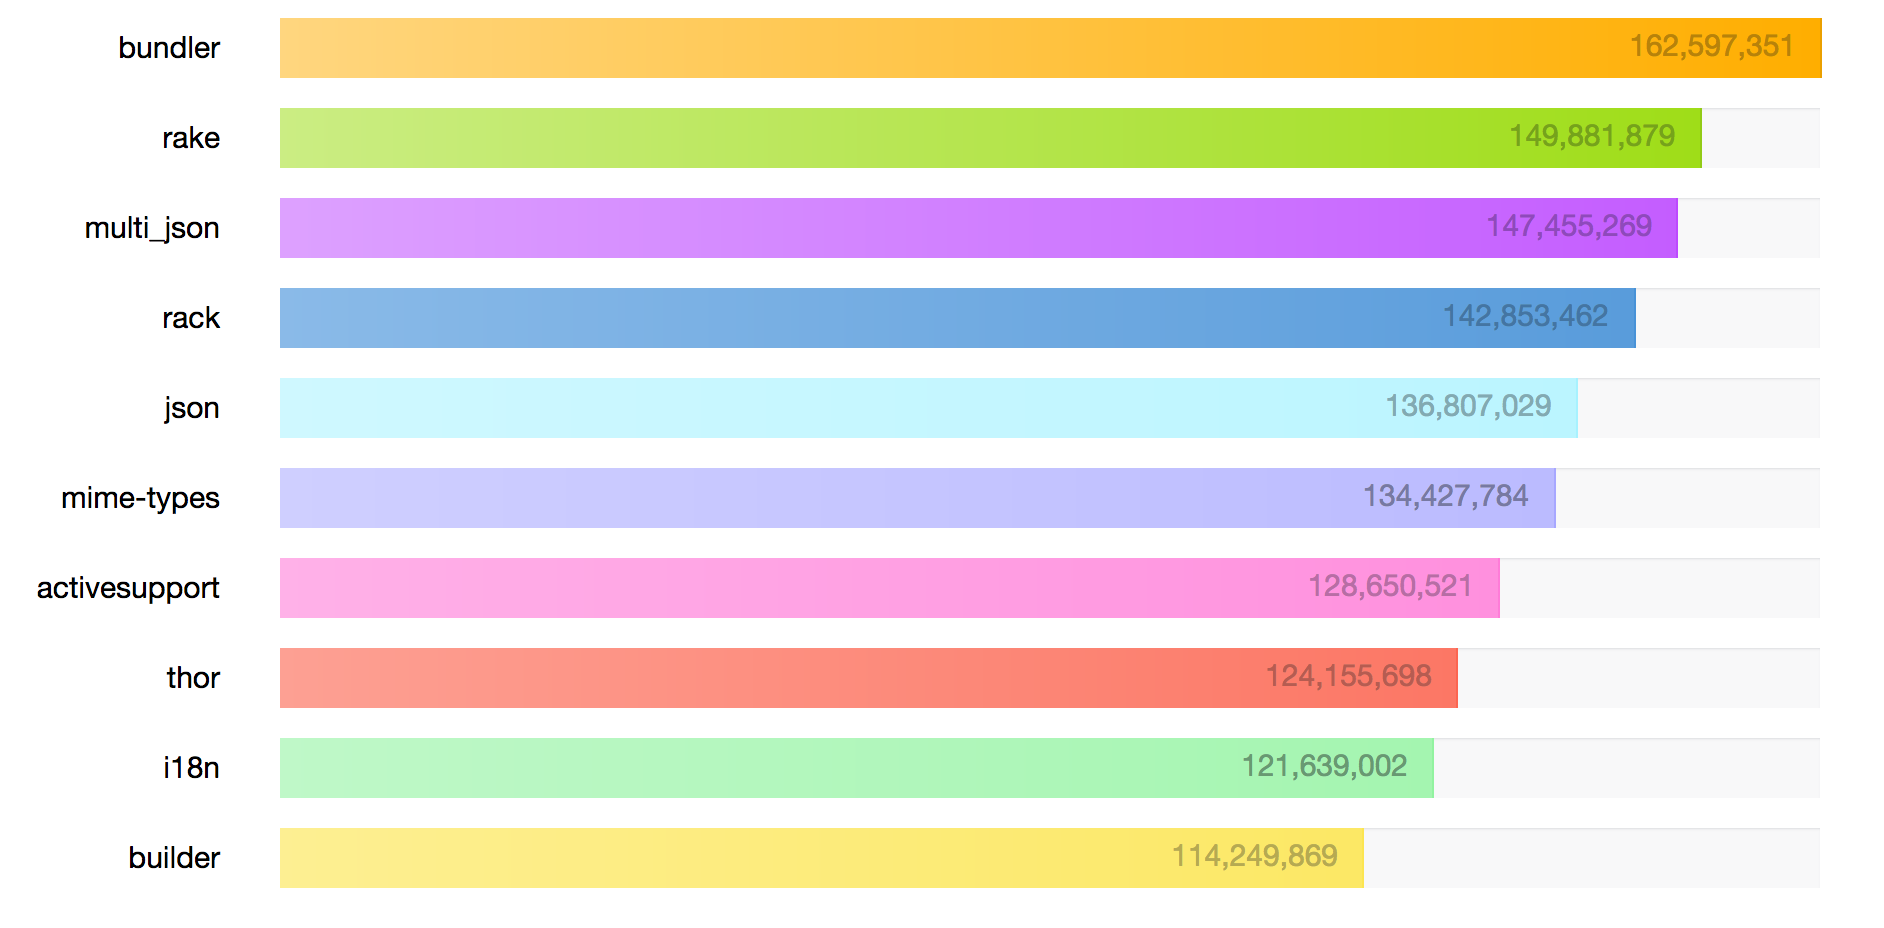
\includegraphics[width=\linewidth]{images/bundler_stats}
  \caption{Statystyki pobrań menedżera pakietów bundler.\\Źródło: \url{https://rubygems.org/stats}}
  \label{fig:bundler_stats}
\end{figure}

Jak widać, \textit{bundler} jest najczęściej pobieranym \textit{gem'em} spośród wszystkich, z ilością pobrań przekraczającą 162,5 miliona. Ogromny wpływ na taki wynik mają oczywiście Rails'y. Strona \url{https://rubygems.org/}, która jest źródłem większości bibliotek, w statystykach podaje, że dostępnych jest ponad 131,600 paczek. Pokazuje to jak ważną częścią dla twórców Ruby on Rails i całej społeczności jest możliwość tworzenia rozszerzeń oraz ich dostępność.

\section{Phoenix} % https://media.pragprog.com/titles/phoenix/intro.pdf   http://www.phoenixframework.org/docs/resources

\textit{Phoenix} jest open source'owym frameworkiem webowym napisanym w języku \textit{Elixir}. Inicjatorem tego projektu jest amerykanin Chris McCord. Pierwsza wersja \textit{Phoenix'a} została wydana 28 sierpnia 2015 roku, a więc jest to bardzo młody framework. Pomimo swojego młodego wieku, framework ten zyskał sporą popularność i zainteresowanie społeczności. Jest to spowodowane ideą frameworku, który nie stara się być na siłę inny od istniejących rozwiązań, a zamiast tego stara się wykorzystywać ich najlepsze elementy. Jako przykładowe frameworki, z których czerpie \textit{Phoenix}, wymieniane są \textit{Ruby on Rails} oraz \textit{Django} \cite{phoenix_docs}.

Tak, jak większość frameworków webowych, \textit{Phoenix} implementuje wzorzec \textit{Model-View-Controller}.

\subsection{Podstawowe założenia}
Idea działania \textit{Phoenix'a} opiera się na kilku podstawowych założeniach:
\begin{itemize}
  \item szybkość działania,
  \item współbieżność,
  \item wygoda użytkowania,
  \item niezawodność.
\end{itemize}

\subsubsection{Szybkość działania}
Położenie nacisku na szybkość działania aplikacji stworzonej przy pomocy frameworka jest czymś naturalnym. Zwykle jednak szybkość działania osiągana jest kosztem innych aspektów tworzenia aplikacji, jak na przykład szybkością powstawania oprogramowania. Aby osiągnąć zadowalającą szybkość działania, twórcy \textit{Phoenix'a} zdecydowali się stworzyć framework przy pomocy języka \textit{Elixir}. Wpływ tego języka na framework opisany jest szerzej w sekcji \ref{phoenix:elixir}.

Poza samym językiem programowania, na szybkość działania aplikacji wpływ mają następujące rozwiązania:
\begin{itemize}
  \item router kompilowany jest do bardzo szybkiego w działaniu \textit{pattern matching'u}, czyli dopasowaniu do wzorca. Dzięki temu optymalizacja wydajności wykonywana jest jeszcze zanim zapytanie opuści router,
  \item template'y są prekompilowane, \textit{Phoenix} nie musi kopiować łańcuchów tekstowych dla każdego wyświetlanego template'u, przez co możliwe jest bardzo wydajne cache'owanie.
\end{itemize}

\subsubsection{Współbieżność}
Wraz z rozwojem możliwości sprzętowych, a dokładniej z rosnącą liczbą rdzeni procesorów, możliwe jest coraz większe wykorzystanie współbieżności w aplikacjach internetowych. Większość frameworków opartych jest na językach obiektowych, co niestety generuje problemy w kwestii współbieżności. Jest tak, ponieważ aby skorzystać z mechanizmu współbieżności, programista musi taką funkcjonalność zaimplementować, oczywiście przy pomocy dostępnych w języku narzędzi. Niestety, współbieżność nie jest prostym zagadnieniem, posiada wiele pułapek, przez co programiści, jeśli nie muszą, zwykle z niej nie korzystają.

Współbieżność, podobnie jak szybkość działania, jest cechą, która osiągnięta została poprzez wybór odpowiedniego języka programowania. \textit{Elixir}, jako język funkcyjny stworzony do tworzenia bardzo wielu procesów, w pełni spełnia wymogi stawiane przez twórców \textit{Phoenix'a}. Nie tylko posiada on bardzo wydajne mechanizmy zapewniające współbieżność, ale przede wszystkim bardzo ułatwia korzystanie z owej współbieżności. I owe ułatwienie pracy programisty jest ważnym czynnikiem popularności \textit{Phoenix'a}. Przykład łatwości korzystania z mechanizmu współbieżności znajduje się na listingu \ref{lst:phoenix_concurrency}, który pochodzi z pozycji literaturowej \cite{phoenix_doctrine}.

\begin{lstlisting}[label={lst:phoenix_concurrency}, caption=Współbieżność w Phoenix'ie]
company_task = Task.async(fn -> find_company(cid) end)
user_task = Task.async(fn -> find_user(uid) end)
cart_task = Task.async(fn -> find_cart(cart_id) end)

company = Task.await(company_task)
user = Task.await(user_task)
cart = Task.await(cart_task)
\end{lstlisting}

Dzięki tak prostym interfejsom, wykonanie kodu z listingu \ref{lst:phoenix_concurrency} zajmie tyle, ile najdłuższe zapytanie do bazy danych, a nie łączny czas zapytań. Dzięki temu dużo lepiej wykorzystywana jest baza danych, co przekłada się na szybkość działania całej aplikacji.

\subsubsection{Wygoda użytkowania}
Wygoda użytkowania jest wypadkową wielu czynników. Z jednej strony jest to wybrany język programowania, który udostępnia programiście w przystępny sposób wiele zaawansowanych mechanizmów, ma ,,przyjazną'' składnię i jest dość prosty w nauce. Z drugiej strony \textit{Phoenix} w swoich założeniach chce się wzorować na innych frameworkach wykorzystując ich najlepsze elementy. Tak więc programista korzysta z rozwiązań, które mogą być mu znane z innych technologii, jak na przykład \textit{Django} lub \textit{Laravel}, co dodatkowo przyspiesza powstawanie aplikacji webowych.

\subsubsection{Niezawodność}
Niezawodność jest podstawą każdej aplikacji, nie tylko internetowej. Nawet najładniejszy, współbieżny i responsywny kod jest bezwartościowy, jeśli nie jest niezawodny. Aplikacje pisane w \textit{Erlang'u} zawsze były bardziej niezawodne od innych, głównie poprzez strukturę linkowania procesów oraz komunikację pomiędzy procesami, co pozwala na efektywną pracę \textit{supervisor'a} \cite{phoenix_doctrine}.

Po raz kolejny jedno z głównych założeń frameworka jest głęboko zakorzenione w przeznaczeniu języka programowania. Wysoka niezawodność jest oczywiście celem praktycznie wszystkich aplikacji, ponieważ błędy aplikacji są bardzo kosztowne dla ich właścicieli.

Dla programistów niezawodność fundamentów, na których budują funkcjonalność aplikacji, jest nieoceniona. Dużo łatwiej tworzy się aplikację mając pewność, że abstrakcje nałożone przez framework są wydajne i niezawodne, przez co można skupić się na tworzeniu funkcjonalności.

\subsection{Elementy składowe}
\textit{Phoenix} jest nadrzędną warstwą w wielowarstwowym systemie zaprojektowanym, aby być modularnym i elastycznym. Pozostałe warstwy zawierają narzędzia takie jak \textit{Plug} (odpowiedzialny za modularność), \textit{Ecto} (odpowiedzialny za interakcję z bazą danych), \textit{Cowboy} (serwer HTTP Erlanga) \cite{phoenix_docs}.

Efektem połączenia wszystkich warstw są następujące elementy:
\begin{itemize}
  \item \textbf{endpoint}, który jako pierwszy zajmuje się zapytaniami, odpowiednio je obsługuje i przekazuje do routera,
  \item \textbf{router} - parsuje przychodzące zapytania i przekierowuje je do odpowiednich kontrolerów i akcji,
  \item \textbf{kontroler} - dostarcza on akcje, które obsługują zapytanie (przetwarzanie danych, przekazanie ich do widoków, generowanie HTML przekazywanych do przeglądarki),
  \item \textbf{szablony} - w połączeniu z danymi oraz po pewnym przetworzeniu generują widoki,
  \item \textbf{widoki}, które są warstwą prezentacji, czyli wizualnym efektem działania aplikacji,
  \item \textbf{kanały} - zarządzają websocketami, które umożliwają komunikację w czasie rzeczywisttym pomiędzy serwerem, a klientem.
\end{itemize}

\subsection{Język programowania - Elixir} % https://elixir-lang.org/
\label{phoenix:elixir}
Podobnie, jak w przypadku \textit{Ruby on Rails}, duży wpływ na jakość użytkowania \textit{Phoenix'a} ma język programowania, w którym jest on stworzony. \textit{Elixir} jest kompilowanym językiem funkcyjnym, który uruchamiany jest na maszynie wirtualnej \textit{Erlanga}. Dodatkowo, jak piszą jego twórcy, jest językiem programowania zaprojektowanym do tworzenia skalowalnych i łatwych w utrzymaniu aplikacji \cite{elixir}.

Wybór tego języka programowania umożliwia zrealizowanie jednych z podstawowych zadań \textit{Phoenix'a} - zapewnienie wysokiej wydajności oraz niezawodności.

Dodatkowo twórcy zwracają uwagę na przyjazną składnię, co stanowczo ma wpływ na popularność frameworka. Jest tak, ponieważ programiści zwykle wolą czerpać przyjemność z używania ,,ładnego'' języka, niż uczyć się i używać mało przyjaznego języka programowania. \textit{Elixir}, jako pierwszy funkcyjny język programowania, wspiera makra z rodziny języków \textit{Lisp}, lecz robi to stosując bardziej naturalną składnię \cite{phoenix_doctrine}.

\subsection{Pozostałe cechy}
\subsubsection{Biblioteki}
Idea centralnego repozytorium paczek jest bardzo popularna wśród większości języków programowania. Ułatwia ono pracę w aplikacją, dodawanie nowych zależności nie jest problematyczne, a błędy dotyczące niezgodności wersji zależności są wyeliminowane. Dla języka \textit{Elixir} domyślnym menadżerem paczek jest \textit{Hex}.

\begin{figure}[h]
  \centering
  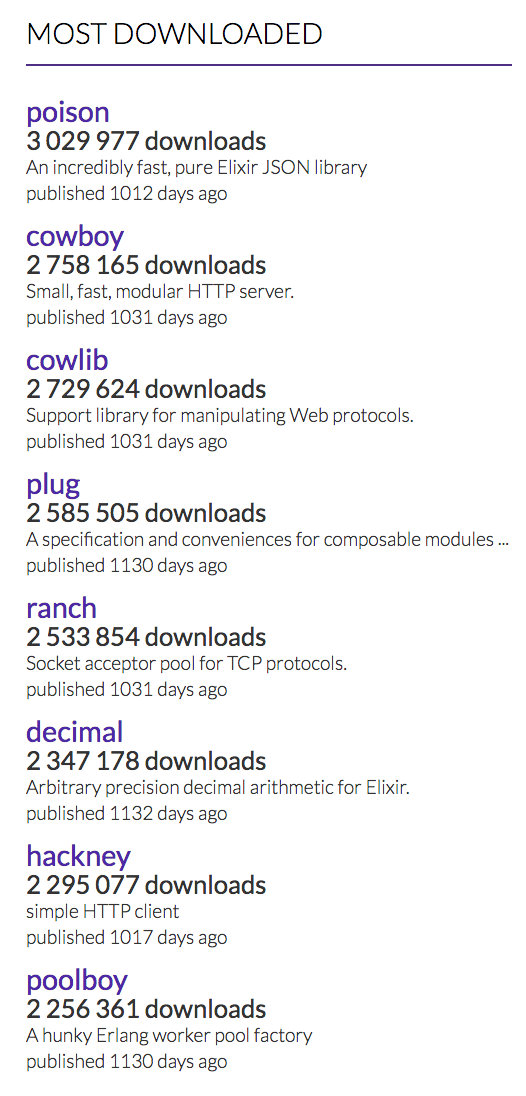
\includegraphics[width=.4\linewidth]{images/hex_stats}
  \caption{Statystyki pobrań menedżera pakietów Hex.\\Źródło: \url{https://hex.pm/}}
  \label{fig:hex_stats}
\end{figure}

W momencie powstawania niniejszej pracy, dostępnych jest ok 4,5 tysiąca bibliotek w oficjalnym repozytorium  \textit{Hex}. W porównaniu do innych, będących na rynku dłużej języków i frameworków, jest to niewielka liczba. Biorąc natomiast pod uwagę rosnącą popularność \textit{Phoenix'a}, można założyć iż ta liczba będzie rosnąć. Obecnie istniejące paczki są niekiedy odpowiednikami istniejących już paczek napisanych w innych językach. Niestety, bardzo często paczki te, z racji na krótki okres istnienia, są mocno niedopracowane.

\section{Express}
\textit{Express} jest minimalistycznym i bardzo elastycznym frameworkiem webowym. Framework ten powstał poprzez dostarczenie wrapperów dla API udostępnianego przez platformę \textit{Node.js}. \textit{Express}, ze względu na swoją budowę, można traktować jako podstawę do budowy innych frameworków. Framework ten jest dostępny jako wolne oprogramowanie pod licencją MIT i komercyjnie wspierany jest przez firmę \textit{StrongLoop}. \textit{Express} nie jest frameworkiem typu \textit{full-stack}, jest on nastawiony na możliwość dowolnej konfiguracji zależności niezbędnych w projekcie.

\subsection{Podstawowe założenia}
% http://noeticforce.com/best-nodejs-frameworks-for-web-and-app-development
% Sinatra inspired!!!
Pierwotną ideą powstania \textit{Express'a} była chęć stworzenia frameworka podobnego do istniejącego w języku programowania \textit{Ruby} frameworka \textit{Sinatra}. Z tego względu oba te frameworki współdzielą podejście do rozwiązywania problemów oraz struktury kodu.

\subsubsection{Configuration over convention}
Głównym założeniem frameworka \textit{Express} jest dostarczenie programistom pełnej elastyczności i możliwości wyboru poszczególnych składowych aplikacji. W skład frameworku nie wchodzą więc biblioteki odpowiedzialne m.in. za:
\begin{itemize}
  \item komunikację z bazą danych,
  \item autentykację użytkowników,
  \item silnik szablonów.
\end{itemize}

Zastosowanie podejścia \textit{configuration over convention} może być problematyczne w przypadku rozpoczynania swojej przygody z \textit{Express'em}. W sytuacji, kiedy framework nie dostarcza wbudowanych mechanizmów, jak np. wcześniej wymieniony adapter do bazy danych, programista nie znający dostępnych bibliotek może mieć duże problemy z wyborem odpowiedniego mechanizmu.

\subsubsection{Organizacja struktury aplikacji}
Ze względu na podejście \textit{convention over configuration}, \textit{Express} nie narzuca programistom konkretnej struktury aplikacji. W żaden sposób nie jest wyróżnione podejście, które najczęściej można spotkać w aplikacjach webowych, czyli \textit{Model-View-Controller}. Programista może wybrać dowolny wzorzec projektowy, bądź też nie zastosować żadnego, jeśli taka jest jego wola.

\subsection{Podstawa dla innych frameworków}
% typy zbudowanych frameworków + nazwy
\textit{Express} bez żadnych dodatkowych bibliotek, czyli od razu po instalacji, nie dostarcza wielu, niekiedy ważnych, funkcjonalności. Programiści korzystający z tego frameworka potrzebowali jednak tych samych narzędzi w przypadku tworzenia aplikacji tego samego typu. W momencie, kiedy za każdym razem musieli dołączać do projektu i konfigurować te same biblioteki, zaczęły powstawać bardziej ,,kompletne'' frameworki, które bazowały na \textit{Expressie}. W ten sposób powstały następujące frameworki:
\begin{itemize}
  \item LoopBack - stworzony do budowy REST API,
  \item ItemsAPI - framework łączący funkcjonalność \textit{Elastichsearch'a} i \textit{Express'a},
  \item KeystoneJS - \textit{Content Management System},
  \item MEAN - framework typu full-stack,
  \item Feathers - stworzony do budowy REST API,
  \item Sails.js - framework MVC typu full-stack,
  \item Hydra-Express - framework stworzony do architektury mikroserwisów.
\end{itemize}

\subsection{Biblioteki}
Większość języków programowania posiada swój menedżer paczek, nie inaczej jest w przypadku języka \textit{JavaScript}. W tym środowisku największą popularność zyskał \textit{npm}. Jako, że \textit{npm} jest menedżerem paczek języka, a nie frameworka, można tam oczywiście znaleźć paczki niekompatybilne z \textit{Expressem}, lecz jest to cecha wszystkich menedżerów stworzonych dla konkretnego języka programowania.

Na oficjalnej stronie \textit{npm} \cite{npm_site} przeczytać można, że dostępnych jest ponad 470 tysięcy paczek. Z repozytorium \textit{npm} tygodniowo pobieranych jest 2 365 813 490 paczek.
